\chapter{Motivation}

Advances in drone technology in recent years
have opened the door to many application possibilities in the civil sector. \cite{MunichRE}
With regard to the commercial use of drones, 
in the near future great economic potential is expected within the fields of
infrastructure,
transport,
insurance,
media and entertainment,
telecommunication,
agriculture,
safety
and mining. \cite{PwC2016}
In contrast,
more visioniary ideas such as drone delivery
have not been broadly realized yet. \cite{Rosen2019}
Across the globe, many big corporations and smaller start-ups 
are conducting research on drone delivery applications. \cite{Garcia2019}
Until now, only several smaller
test projects in sparsely populated areas have been realized. 
Decisive reasons for this are of a technical nature. 
In particular, autonomous navigation methods are not yet 
robust enough for the reliable deployment in densely populated urban areas. \cite{loquercio2018learning}
This master's thesis is intended to make a contribution to autonomous navigation of drones with basic research on 
integrating temporal comprehension into the navigation method.


In science as well as in this thesis proposal, the colloquial term "drone" refers
to the aircraft class of unmanned aerial vehicles (UAVs).
The International Civil Aviation Organization (ICAO) \cite{ICAO2005} defines UAVs
as aircrafts without a human pilot onboard, which are either remote-controlled by a human operator or "preprogrammed and fully autonomous".
An UAV is a component of an unmanned aerial system (UAS), which additionally consist of a ground control station, communication link and payload. 
Basic components of UAVs are an airframe, an electric power system, a flight
control system and an air data terminal. \cite{Fahlstrom2012}
For UAVs with autonomous functions, onboard computers
provide the required additional computation power.
Various systems exist to classify UAVs either by 
airframe type \cite{Austin2011} or by flight key characterstics \cite{USDOD2011, Wei2016}.
With respect to the latter, 
Watts, Ambrosia and Hinkley \cite{Watts2012} proposed a classification system 
for scientific usage.
Table \ref{tab:UAV_classification_system_by_Watts_Ambrosia_and_Hinkley} shows a selection of the system's UAV sub-classes, 
i.e., micro air vehicles (MAV), low altitude, short endurance (LASE),
low altitude, long endurance (LALE), medium altitude, long endurance (MALE) and
high altitude, long endurance (HALE).
This proposal can be primarly associated with
quadcopters, the representative of MAVs
that, according to my observations, prevails among hobbyists and commercial applications.


UAVs originate from the military, were adopted by
enthusiasts, have gained more and more acceptance in the industry and finally have become today's standard in 
aerial inspection services in
agriculture,
construction,
infrastructure,
utilities,
and mining. \cite{McKinsey, Equinox, Percepto}
With fast aerial maneuverability,
UAVs exhibit several substantial advantages over ground vehicles.
As they are unaffected by many obstacles and largely independent of infrastructure,
destinations can be reached by the shortest route, waiting times can be avoided
and the effort and risk of getting to places that are difficult to access can be reduced. \cite{Watts2012}
In addition, from the privileged perspective of a bird, onboard sensors 
are able to record extensive data of high quality fast at low cost. \cite{PwC2016}
This ability is extremly valuable in the context of big data, cloud computing and machine learning. \cite{Garcia2019}
On the downside,
MAVs are smaller aircraft vehicles that can move substantially less weight
which, besides computational power and mission-specific payload,
limits battery capacity,
which in turn restricts flight range and duration.
For MAVs paying off economically, efficiency is therefore paramount.
A central approach to increase efficiency is to shift functions from a human operator to the drone itself,
i.e., increase the drone's degree of autonomy.
This becomes particularly clear in the example of delivery applications.
Because drones can load significantly fewer packages and
have to recharge more often than conventional delivery trucks have to refuel,
one human pilot per drone would be too ineffective for broad deployment.
Drone delivery systems are only profitable
if most functions are performed autonomously by the individual delivery drone,
or, at best, by the collective of the drone swarm.
Consequently, expensive human labor could be reduced
and vast room for mathematical optimization could be created. \cite{Chiang2019, Lee2017}


So far, UAVs have proven their value in fields that are connected with large industrial sites which usually
provide flight environments that are essentially demarcated and controlled and therefore very predictable.
State-of-the-art autonomous drones are capable of dealing with these environments.
Here, mention can be made
of drone-in-a-box systems:
the box provides takeoff/landing and charging infrastructure for
the drone or drone swarm, that autonomously execute preprogrammed flight missions. \cite{drones5040108}
In comparison,
the open-world environments of 
our daily lives 
are densely disturbed and are, thus, characterized by high uncertainty.
Drones have not yet asserted themselves for 
commercial applications in these environments.
This is particularly true for drones with
autonomous functions.
Crucial reasons for this are
legal restrictions, lack of acceptance
and technical complexity, 
notably with respect to "navigation, communication and automatization"\cite{kellermann2020drones}. \cite{Rosen2019}


Autonomous navigation is a highly relevant topic in current UAV-related public research.
Navigation, which is a basic functionality of each UAV,
comprises the main task of achieving a desired pose or position
while performing necessary sub-tasks at the same time. \cite{loquercio2018learning}
The necessity of individual sub-tasks depend on the flight environment.
In densely populated open-world areas an autonomous navigation method should integrate
functions to handle
obstacle avoidance and the coordination with other agents,
while in rural areas or on controlled industrial sites 
navigating through pre-planned waypoints only relying on global navigation satellite system (GNSS) sensors may be sufficient.
Current autonomous navigation methods lack in robustness for complex environments and do not exhaust the full agility of MAVs.


%Consequently, 
%whether the state of the art in autonomous navigation of UAVs
%is sufficiently robust depends on the flight environment and the flight mission.
%Again, drone delivery provides an explanatory example here.
%Projects have been already 
%realized in rural areas where the airspace is mainly undisturbed [].
%Here, navigating through waypoints only relying on GNSS 
%without any implementation of obstacle avoidance and agent-coordination may be sufficient. 
%In contrast, urban areas are full of unstructered obstacles and other participating agents 
%which result in a high uncertainty that cannot be faced with in-advance planning. 
%Only a high level of autonomy in navigation
%could robustly cope with the challenges of this environment.
%This level has not yet been achieved.


%Research on autonomous MAV navigation mainly relies on deep learning 
%which allows to comprehend the immediate environment based on the perception of
%onboard sensors. \cite{loquercio2018learning}
%State-of-the-art navigation methods 
%achieve a high spatial understanding of the environment
%by feeding convolutional neural networks with RGB or depth data.
%This research aims to develop a simple navigation method 
%that extend this spatial perception onto temporal extension 
%by serially connecting a CNN with a long-short-term-memory (LSTM) network.
%Based on my assumption that powers of recall are crucial for humans when navigating,
%I am convinced that future autonomous navigation systems will also encompass this ability.
%The navigation method will be tested in simulation and real world in a simplified test scenario,
%which, however, requires the MAV to remember the expansion and relative motion of obstacles while considering its own elapsed acceleration.




\chapter{Objectives}

Public research has put forth many advanced methods for autonomous navigation of MAVs.
However, they are not sophisticated enough to conquer open-world environments of high uncertainty
such as urban areas. \cite{loquercio2018learning}
In current research, deep learning techniques that empower MAVs with comprehension abilities
constitute the best approach to face the uncertainty of these environments.
State-of-the-art navigation methods 
integrate feedforward, deep convolutional neural networks
that map the current color or depth image to action.
Thereby a high, spatial comprehension
of the immediate surrounding of the MAV can be achieved.
But I suspect that the mere understanding of space, as good as it may be,
is not enough for the autonomous navigation of MAVs
in open-world environments.
Therefore, I aim to develop a navigation method that besides spatial also includes temporal comprehension.
The following objectives should be achieved within the scope of the master's thesis.


The method is intended to expand the work of Kaufmann et al. from ETH Zurich in 2018 \cite{Kaufmann2018}.
They developed a vision-based navigation method that enables a drone to fly autonomously 
through a drone race track, thereby
achieving high reliability with high speed and agility on dynamic flight curves. 
Their hybrid approach consists of a convolutional neural network (CNN) and a conventional control system that repeatedly executes the following steps at a high frequency:
Inputting the current raw RGB image from the onboard, forward-facing camera, the CNN generates a waypoint in the 2D reference frame of the image ($x, y \in [-1, 1]$).
The waypoint is transformed from the reference frame of the image to the reference frame of the drone state estimation ($x, y, z \in \mathbb R^3$). 
A trajectory from the current drone state estimate to the waypoint is computed by minimizing jerk, which is the time derivative of acceleration.
The states of the trajectory are then tracked by a conventional control algorithm.
The end state of the trajectory is never reached since the re-planning of the trajectory is continually triggered by new waypoints.
In my thesis I plan to make progress on the first part of the hybrid approach 
by adding a recursive network to the CNN (CNN-LSTM).
Furthermore, I would like to examine if feeding additional features (e.g., state estimates) to the network is beneficial.
I expect that thereby, 
waypoints are not only generated on the basis of the current RGB image, 
but that also past images (and possibly also current and past state estimates of the drone) are included in the navigation decision.
This would possibly result in the following positive effects:
\begin{itemize}
	\item Due to its "memory", the network is able to generate meaningful waypoints in case that the next gate of the race track is not depicted in the current image, but has appeared in previous images.
	\item Due to temporally distributed images, the network is able to take the speeds of moving gates (or obstacles) into the account of the navigation decisions.
	\item Since trajectories are temporally extended maneuvers, a network with temporal comprehension is more able to imitate the expert policy.
	Thus, the resulting trajectory through the race track formed by the successively generated waypoints is more similar to a precomputed optimal (in terms of acceleration, jerk, snap, ...) trajectory.
\end{itemize}
The approach is implemented utilizing the middleware ROS \cite{ros}
and simulated with the photo-realistic Flightmare Simulator \cite{song2020flightmare}.
Tests to compare my extended approach with the original method should be designed
and conducted to investigate if the above enhancements could be realized.



My work is based on the paper of Kaufmann et al. \cite{Kaufmann2018} from 2018.
Just recently, follow-up work from ETH Zurich \cite{Loquercio2021Science} with 
a way more sophisticated autonomous navigation method has been published. 
The neural network is designed to cover a bigger scope
by directly outputting trajectories instead of waypoints in image coordinates.
However, I intend to still base my work on the earlier paper,
since the more modular design provides a very good starting point with respect to my intended basic research
whether temporal comprehension leads to improvements in autonomous navigation.
Moreover, the test environment of drone racing is very convenient due to its simplicity.
The completion of the race track can be achieved by mere reactive control to the next gate
and does not require the formulation of a high level navigation goal
whose implementation would pose another challenge.




%- As mentioned above, the navigation method theoretically does not require a high-level goal formulation
%since the reactive targeting the next gate already results in completing the race track.
%Practically, in the event that at any time the next gate is not located 
%in the frame of view (FOV) of the MAV's onboard camera,
%the output of the deep neural network (DNN) is not defined and the lack of a high-level goal becomes evident.
%This is also the case, even if the MAV has seen the next gate in the past (see figure ??).

%- In addition, humans cannot estimate the velocity and direction of motion of themselves, obstacles or other agents
%based on a short blink with their eyes but they need to observe over at least a short period of time.
%- Not only localization but also situational reasoning is strengthened by memory,
%e.g., a car driver observes a child that runs from the sidewalk through the parking cars onto the road
%and has enough reaction time or even anticipation to brake.
%Without any power of recall, the driver may start braking in anticipation
%when the child is still on the sidewalk, but may stop braking after the child disappears behind a parking car.
%
%- dynamic trajs

%In the navigation method of this research, I want to meet the lack of high-level goal planning 
%by introducing powers of recall to navigation.
%To my knowledge, Kelchtermans and Tuytelaars \cite{Kelchtermans2017}
%are the only ones who used a recurrent neural network for memory abilities in autonomous, 
%vision-based UAV navigation. \cite{Shakeri2019}
%-reason why their work is not what i want..
%However, they only tested their method in simulation and did not comprehensively evaluate their results.
%If the method, after passing the first gate, could remember that it has seen the second gate before,
%the method could plan to navigate through the second gate based on elapsed images.

%In my method, I plan to use a LSTM-CNN which is a deep convolutional neural network
%serially connected to a long-short-term-memory (LSTM) neural network.
%
%While the CNN has the ability to perceive and reason spatial structures of the immediate environment,
%the LSTM is able to establish connections through time. 
%
%In other words, the CNN is responsible to predict waypoints 
%or generate trajectories based on single images,
%whereas the LSTM empower the method to recall and remember 
%by evaluating the temporal structure between the predictions of the CNN.
%
%Besides the above steep curve scenario, this memory would show great benefit in situations
%when the quadcopter lost track of the goals and it can recall elapsed images.
%In case of the application in urban areas, for example, 
%quadcopters could remember obstacles 
%that were visible but have become occluded and thus, could better anticipate. 
%Or after an evasive maneuver, 
%the quadcopter could return to the actual path 
%much faster because he memorizes its maneuver.
%In that sense, the memory of the quadcopter is another form of localization in the environment, 
%which is not global but namely local.
%In addition, memory could enable better optimization, e.g., 
%the imitation learning of optimal trajectories which
%are not only spatial but also temporal objects.
%However, this research, in a simplified scenario, should only prove if powers of recall 
%are applicable and generally useful for the autonomous navigation of MAVs.

\chapter{Task Packages}
Based on the objectives, the following task packages are defined:

\begin{itemize}
	\item Build the drone racing simulation.
	\begin{itemize}
		\item Familiarize with Flightmare \cite{song2020flightmare}, a photo-realistic simulator for quadcopters.
		\item Familiarize with the Unity Engine \cite{Unity}, to create and manipulate the rendered environments in Flightmare.
		\item Transfer the already implemented simulation from Gazebo \cite{Koenig2004} to Flightmare.
	\end{itemize}
	\item Generate training data in simulation.
	\begin{itemize}
		\item Adjust already implemented expert policy, so that the training data includes additional features and labels.
		\item Run simulation to generate the data.
	\end{itemize}
	\item Build the recurrent convolutional neural network (R-CNN).
	\begin{itemize}
		\item Familiarize with PyTorch \cite{NEURIPS2019_9015}.
		\item Transfer already implemented data input pipeline from TensorFlow \cite{tensorflow2015-whitepaper} to PyTorch.
		\item Familiarize with R-CNNs.
		\item Design the R-CNN using hyperparameters for later adjustments.
		\item Implement the R-CNN in PyTorch.
		\item Train the R-CNN and find best values for the hyperparameters.
	\end{itemize}
	\item Evaluate my approach.
	\begin{itemize}
		\item Design test scenarios for comparison with the base navigation method of Kaufmann et al. \cite{Kaufmann2018}.
		\item Implement and conduct tests in simulation. 
		\item Evaluate results of tests.
	\end{itemize}
	\item Write thesis documentation.
	\item (Optional) Conduct test in real world.
	\begin{itemize}
		\item Implement my approach on real drone.
		\item Find test site and rebuild a test scenario that in simulation produced promising results.
		\item Conduct test, evaluate and document in thesis.
	\end{itemize} 
 
\end{itemize}

	
\chapter{Time Schedule}

\begin{figure}[H]
    \centering
    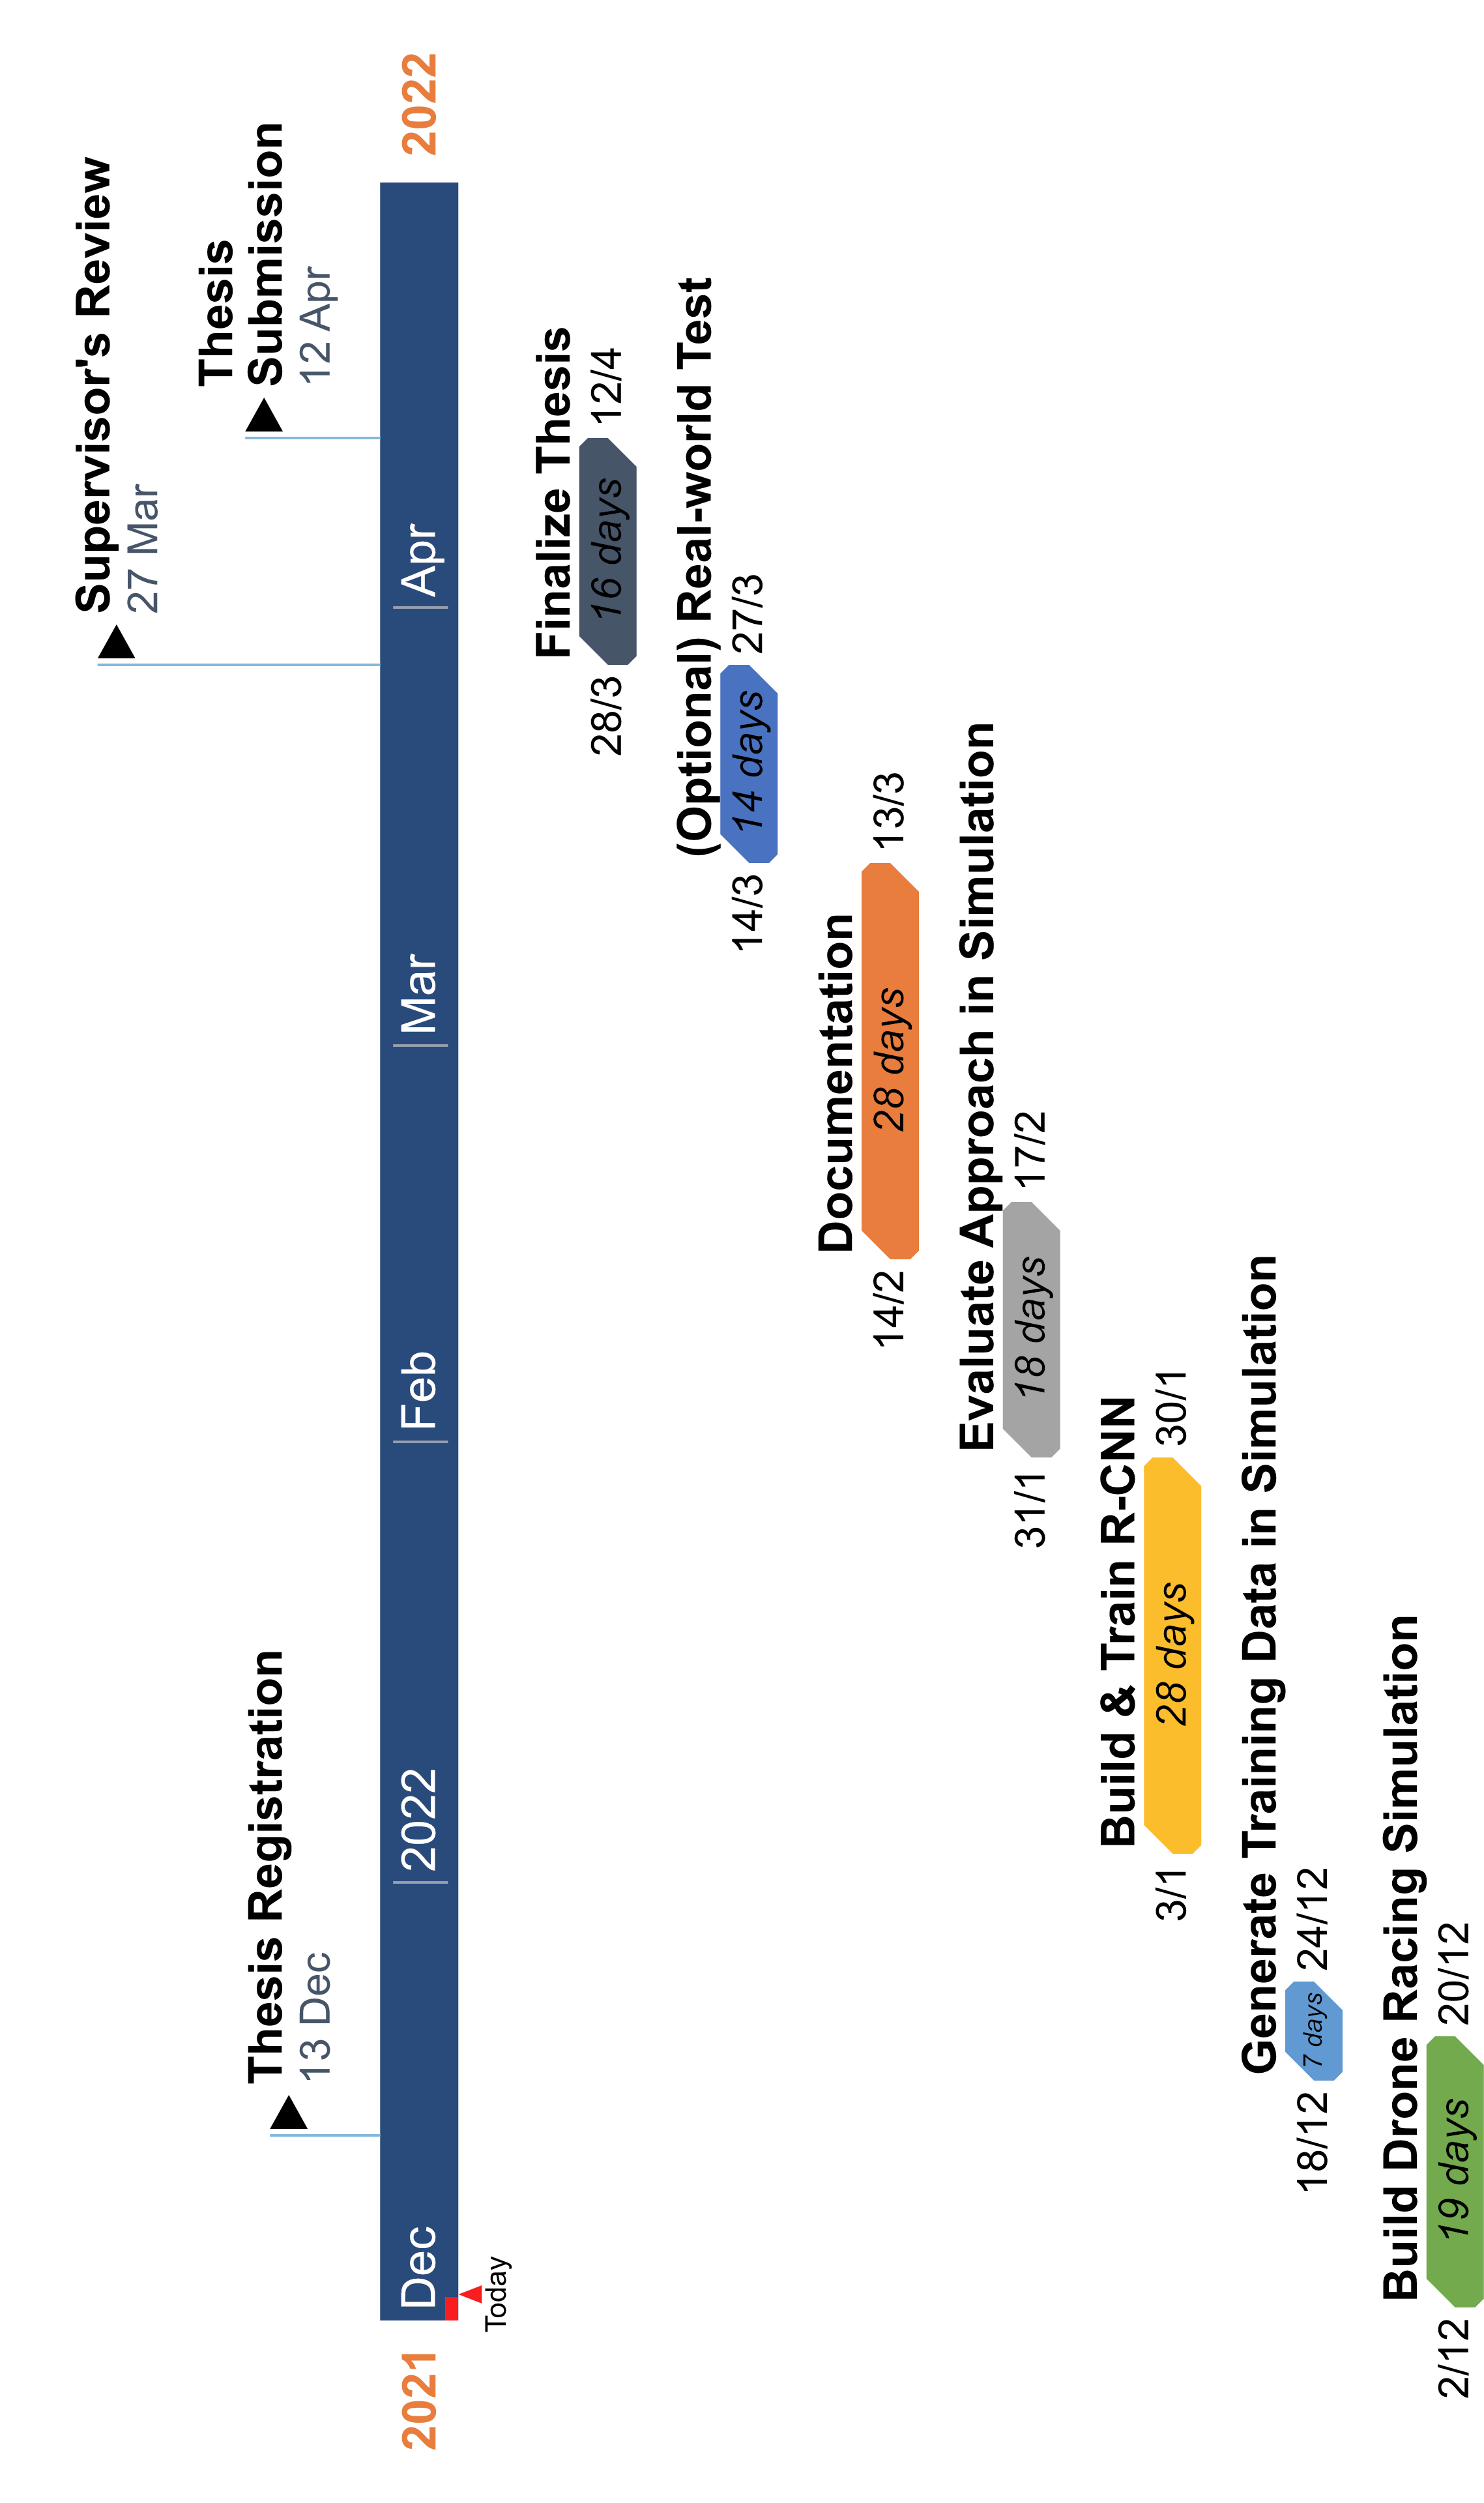
\includegraphics[width=0.6\textwidth]{figures/Timeline.png}
%    \decoRule
    \caption[Gannt diagram illustrating the time schedule of the master's thesis.]{Gannt diagram illustrating the time schedule of the master's thesis. \textit{Created with \href{https://online.officetimeline.com/}{Office Timeline Online}}}
    \label{fig:Timeline}
\end{figure}

\chapter{Organizational Matters}
\begin{itemize}
	\item Language of the thesis: English
	\item Text processing system: LaTeX
	\item Programming languages: C++, Python
	\item Supervisor: Dr. rer. nat. Yuan Xu
	\item Reviewers: Prof. Dr. Sahin Albayrak, Dr.- Ing. Stefan Fricke
\end{itemize}

\chapter{Annex}

\begin{table}[H]
    \caption[Selected UAV Classes of the Classification System by Watts, Ambrosia and Hinkley]{Selected UAV Classes of the Classification System by Watts, Ambrosia and Hinkley. \textit{Source: assembled from \cite{Watts2012}.}}
    \label{tab:UAV_classification_system_by_Watts_Ambrosia_and_Hinkley}
    \centering
    \begin{tabular}{r l l l L{0.3\textwidth}}
    \toprule
    \tabhead{Class} & \tabhead{Altitude} & \tabhead{Endurance} & \tabhead{Range} & \tabhead{Takeoff/Landing} \\
    \midrule
    MAV     & < 330 m       & < 30 min  & < 1 km        & Any small area \\
    LASE    & < 450 m       & < 2 h     & < 10 km       & Human hand, catapult system or runway \\
    LALE    & < 5,000 m     & < 20 h    & < 100 km      & Runway \\
    MALE    & < 9,000 m     & < 40 h    & < 1,000 km    & Runway \\
    HALE    & < 25,000 m    & < 30 h    & < 10,000 km   & Runway \\
    \bottomrule\\
    \end{tabular}
\end{table}

%\section{Steep curve scenario}
%
%For example, a section of the racetrack that consist of two successive gates, in between a steep curve
%could not successfully be navigated through by the method, even if both gates have already appeared on images.
%Before the MAV navigate through the first gate, both gates are in the FOV of the camera.
%After it has flown through the first gate, because the curve is too steep, the second gate is out the FOV 
%and the navigation method has no goal to be achieved.

% Taking a human as example
% HUMAN IN THE DRONE RACETRACK EXAMPLE
%To solve this problem I consider what a human would do in this scenario.
%From a position before entering the gate 1, a human can see gate 1 and 2.
%After he flew through gate 1, he has no visual contact to both gates anymore.
%Yet, he can manage to navigate through gate 2 because he has the ability 
%to remember the position of gate 2 in his body frame. 


